\documentclass[12pt,a4paper]{article} 
\usepackage[utf8]{inputenx} 
\usepackage[spanish]{babel} 
\usepackage[left=2cm,right=2cm,top=2cm,bottom=2cm]{geometry}
\usepackage{scrextend}
\usepackage{marvosym}
\usepackage{pifont} % Generación de símbolos especiales
\usepackage{textcomp}
\usepackage{newpxtext}
\usepackage{newpxmath}
\usepackage[T1]{fontenc} % Codificación de salida    
\usepackage{microtype} % Mejoras de microtipografía en la obtención de PDF (sólo para pdflatex)
\usepackage[hyphens]{url} % Para escritura de URL
\urlstyle{sf} % Estilo de URL sin serifas para que tengan un mejor aspecto
\usepackage{tikz}
% Paquetes para obtener un mayor control de las listas
\usepackage{paralist} % Mayor control de listas
\usepackage{multicol} % Elementos en varias columnas
\usepackage[breaklinks]{hyperref}
\usepackage{graphicx}
\usepackage{caption}

\usepackage{listings}
\usepackage{color}

\definecolor{dkgreen}{rgb}{0,0.6,0}
\definecolor{gray}{rgb}{0.5,0.5,0.5}
\definecolor{mauve}{rgb}{0.58,0,0.82}

\lstset{frame=tb,
  language=Java,
  aboveskip=3mm,
  belowskip=3mm,
  showstringspaces=false,
  columns=flexible,
  basicstyle={\small\ttfamily},
  numbers=none,
  numberstyle=\tiny\color{gray},
  keywordstyle=\color{blue},
  commentstyle=\color{dkgreen},
  stringstyle=\color{mauve},
  breaklines=true,
  breakatwhitespace=true,
  tabsize=3
}

\captionsetup[figure]{labelformat=empty}
\author{Julián García Sánchez \and Iván Illán Barraya \and Alejandro Medina Jiménez \and Javier Monescillo Buitrón}
\title{Implementación de un procesador de lenguajes para la generación de Autómatas de Moore}
\date{\today}
%%%%%%%%%%%%%%

\begin{document}
	
	\maketitle
	
	\begin{figure}[h]
		\centering
		
\includegraphics[width=0.25
		\linewidth]{img/uclm}
		\caption{}
		\label{fig:image004}
	\end{figure}

	\newpage
	\tableofcontents
	\newpage
	
\section{¿Qué es una máquina de Moore?}
	
En Teoría de la computación un \textbf{autómata} o \textbf{máquina de Moore} es un autómata de estados finitos muy particular, la salida en un momento dado sólo depende de su estado en ese instante, mientras que la transición al siguiente estado dependerá del estado en el que se encuentre y de la entrada introducida.
\newline
	
	\begin{figure}[h]
		\centering
		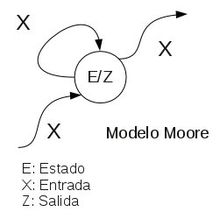
\includegraphics[width=0.5
		\linewidth]{img/modelo-moore}
		\caption{Ejemplo de máquina de Moore simple.}
		\label{fig:modelo-moore}
	\end{figure}
	
Una máquina de Moore \textit{Mmor} se define como una 6-tupla:
	\[ Mmor = (S,S_{0},\Sigma,\Lambda,T,G)  \]
donde definimos los siguientes elementos:
	
	\begin{itemize}
		\item S: es un conjunto finito de estados.
		\item $S_{0}$: es el estado inicial, y además es un elemento de S.
		\item $\Sigma$: un conjunto finito llamado alfabeto de entrada.
		\item $\Lambda$: un conjunto finito llamado alfabeto de salida.
		\item $T$ : una función de transición $T: S \times \Sigma \rightarrow S$ que mapea un estado y una entrada al siguiente estado.
		\item $G$ : una función de salida $G : S \rightarrow \Lambda $ que mapea cada estado al alfabeto de salida.
	\end{itemize}
\clearpage

\newpage

\section{Descripción del problema}
El problema que se presenta es la construcción de un procesador de lenguajes cuya entrada consista en un lenguaje de dominio específico en el cual se declaran una o varias máquinas de Moore. Este lenguaje se ha definido como \textbf{Moor}. La salida del procesador de lenguajes consistirá en uno o varios ficheros generados en un lenguaje de alto nivel, se ha elegido Java por su facilidad de aprendizaje y rendimiento .

\section{Solución propuesta}
Para diseñar dicho procesador de lenguajes, utilizaremos los conocimientos de la materia durante las distintas etapas del proceso.

\begin{itemize}
	\item Diseño del procesador de lenguajes
	\item  Diseño de la fase de análisis \begin{itemize}
		\item Analizador Léxico
		\item Analizador Sintáctico
		\item Analizador Semántico	
	\end{itemize}
	\item Diseño de la fase de síntesis \begin{itemize}
		\item Generación de archivos en lenguaje objeto
	\end{itemize}
\end{itemize}
La primera etapa consta del diseño referente al lenguaje fuente, procesador de lenguajes, o arquitectura general del sistema. Mediante el uso de diagramas tipo T se explicará el funcionamiento del mismo, se proporcionará un diagrama total del problema.
\section{Diseño del procesador de lenguajes}
\begin{figure}[h]
	\centering
	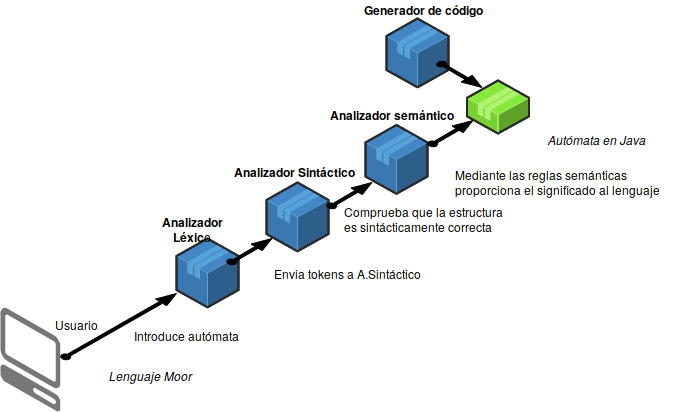
\includegraphics[width=0.7\linewidth]{img/disenio}
	\caption{}
	\label{fig:disenio}
\end{figure}

\clearpage

\subsection{Diagrama tipo T asociado}
Se diseña la construcción del procesador con los diagramas \textbf{tipo T}, de una forma más gráfica se explica el funcionamiento del procesador que se pretende implementar.\newline
El lenguaje fuente será \textbf{Moor} y el lenguaje de salida será \textbf{Java}, el lenguaje sobre el que se implementa también será Java, es decir, el compilador compilará usando Java y se interpretará en otro lenguaje resultante que se denomina \textit{bytecode} gracias a la \textit{JVM}.\newline \newline
\textbf{Java} tiene la particularidad de ser un tipo de lenguaje que es compilado e interpretado.
\newline
Para poder compilar el lenguaje se hace uso de otro compilador auxiliar, que está escrito en código máquina para dar lugar a bytecode, el archivo resultante será un \textbf{.class} que \textit{javac} genera al compilar un archivo fuente \textbf{.java}.
\newline

	\begin{figure}[h]
		\centering
		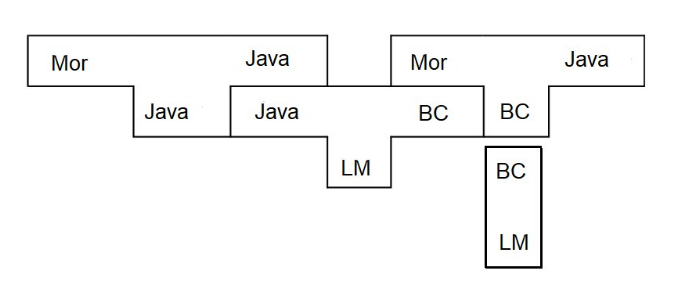
\includegraphics[width=0.7
		\linewidth]{img/T.png}
		\caption{Diagramas tipo T.}
		\label{fig:modelo-moore}
	\end{figure}

\subsection{Lenguaje fuente}
El lenguaje \textbf{Moor} consta de dos secciones principales:

\begin{itemize}
	\item Sección de declaración de código
	\item Sección de declaración de autómatas
\end{itemize}

La \textit{zona de declaración de código} es la parte donde se asignará un comportamiento a un código ya predefinido o que se vaya a ejecutar. Por la forma en la que se ha definido el lenguaje, esta zona será como una zona de \textit{imports} conocida en lenguajes de alto nivel. 
\newline
\newline
La estructura de esta zona es: c$N$ $\#$ \textit{código} $\#$
 donde c es el comportamiento, $N$ es el número de comportamiento y los \textbf{tokens} $\#$ son los delimitadores del código. \newline La característica principal de esta zona es que solo se podrán realizar este tipo de declaraciones, ya que en la otra zona solo podremos declarar autómatas.

\begin{center}
	Ejemplo : c1 $\#$ print('hola') $\#$
\end{center}

Respecto a la \textit{zona de declaración de autómatas} se tendrá una serie de palabras reservadas que se utilizarán para la definición del autómata. No obstante en esta zona solo se podrán declarar autómatas y las funciones asociadas a los mismos, también, como en cualquier lenguaje de alto nivel, se podrán incluir todo tipo de  comentarios '//' o '/$\ast$ Texto comentario '$\ast$/'.
\newline 
\newline
Será posible la declaración de múltiples autómatas en el fichero de prueba, además, se indicará en una tabla todos los campos que son imprescindibles para la realización del mismo.
Cualquier otro carácter introducido en el fichero de prueba será considerado como error.

\subsection{Tabla de Token-Acción}
 En esta tabla se describen tanto los tokens que componen nuestro lenguaje, como la función de cada uno de ellos.

\begin{center}
\begin{tabular}{|c|c|}
	\hline 
	\textbf{Token} & \textbf{Acción} \\ 
	\hline 
	moore & Función para declarar un autómata seguido de un nombre   \\
	& que se escribirá entre llaves $\{\}$ moore Ejemplo $\{\}$\\
	\hline 
	estados & Indica la cantidad de estados totales que tendrá el autómata  \\
	& puede ser un único estado o varios separados por ',' estados q0,q1;\\ 
	\hline 
	estado\_in & Se selecciona un único estado inicial  \\ 
	& que tendrá que estar en los estados anteriores estado\_in q0; \\
	\hline 
	alf\_in & La entrada o eventos del autómata que hará posible las transiciones\\
	& entre estados, único o entre comas ',' alf\_in a,b,c;\\
	\hline 
	alf\_out &  La salida o comportamientos del autómata  \\
	& y tendrán que ser coincidentes con \\ 
	& la zona de declaración de comportamientos, \\
	&  escrito un identificador único o entre comas ',' \\
	\hline
	transicion & Será un tipo de función que se escribirá entre llaves $\{\}$, \\
	& y permitirá que se transite mediante una entrada de un estado a otro: \\ 
	& (<estado\_origen>, entrada, <estado\_destino>); \\
	& se podrán indicar varias mediante el uso de comas ',' \\
	\hline 
	comportamiento & Será un tipo de función que se escribirá entre llaves $\{\}$,   \\ 
	& y permite asignar a un estado un comportamiento: \\
	& (<estados>,<comportamiento>); \\
	& se podrán indicar varios mediante el uso de comas ','\\
	\hline  
\end{tabular} 
\end{center}
Notese, que para cerrar una sentencia es necesario de indicar al final de dicha sentencia el carácter ';', esto no es necesario para las funciones \textit{moore}, \textit{transicion} y \textit{comportamiento}.
JULIAN


\clearpage
\subsection{Tabla de tokens}
En la siguiente tabla de tokens, se muestran los lexemas de ejemplo, los tokens y las expresiones regulares asociadas a cada token.
\begin{center}
		\begin{tabular}{|c|c|c|}
			\hline 
			\textbf{Token} & \textbf{Lexema} & \textbf{Patrón} \\ 
			\hline 
			moore & moore & m$\cdot$o$\cdot$o$\cdot$r$\cdot$e  \\ 
			\hline 
			estados &estados & e$\cdot$s$\cdot$t$\cdot$a$\cdot$d$\cdot$o$\cdot$s \\ 
			\hline 
			estado$\_$in & estado$\_$in & e$\cdot$s$\cdot$t$\cdot$a$\cdot$d$\cdot$o$\cdot$$\_$$\cdot$i$\cdot$n \\ 
			\hline 
			alf$\_$in	& alf$\_$in & a$\cdot$l$\cdot$f$\cdot$$\_$i$\cdot$n \\ 
			\hline 
				alf$\_$out	& alf$\_$out & a$\cdot$l$\cdot$f$\cdot$$\_$o$\cdot$u$\cdot$t \\ 
			\hline 
				transicion	& transicion & t$\cdot$r$\cdot$a$\cdot$n$\cdot$s$\cdot$i$\cdot$c$\cdot$i$\cdot$o$\cdot$n \\ 
			\hline 
				comportamiento	& comportamiento & c$\cdot$o$\cdot$m$\cdot$p$\cdot$o$\cdot$r$\cdot$t$\cdot$a$\cdot$m$\cdot$i$\cdot$e$\cdot$n$\cdot$t$\cdot$o \\ 
			\hline 
			Paréntesis abierto	& ( & ( \\ 
			\hline 
			Paréntesis cerrado	& ) & ) \\ 
			\hline 
			Llave abierta	& $\{$ & $\{$ \\ 
			\hline 
			Llave cerrada	& $\}$ & $\}$ \\ 
			\hline 
			Punto y coma	& ; & ; \\ 
			\hline 
			Coma	& , &  , \\ 
			\hline
			Asterisco barra & $\ast/$  & $\ast$$\cdot/$ \\ 
			\hline 
			Barra asterisco & $/\ast$  &  $/$$\cdot$$\ast$ \\ 
			\hline  
			ID	& hola  & [A-Za-z][A-Zaz0-9$\_$]* \\ 
			\hline 
			CMP	& c1 & c[1-9][0-9]* \\ 
			\hline
		    CODIGO	& $\#$codigo aquí $\#$  & $\#$$\cdot$ codigo aquí $\cdot$$\#$\\ 
			\hline
		\end{tabular} 	
	\end{center}


\subsection{EBNF}
Por último, en la siguiente figura puede ver una representación de la gramática del lenguaje en EBNF.

			\begin{center}
			\begin{tabular}{lcl}
	

				PROGRAMA & ::= & DEC$\_$COMP AUTOMATA $\{$AUTOMATA$\}$ \\ 
				 
				
				DEC$\_$COMP & ::= &CMP  CODIGO $\{$ CMP CODIGO $\}$ \\ 
			
				CODIGO 	&::= &'$\#$' ASCII '$\#$' \\ 
				
				AUTOMATA & ::= & \textbf{moore} ID CUERPO$\_$AUTOMATA \\
				
			
				CUERPO$\_$AUTOMATA	& ::= & $'\{'$ ESTADOS ESTADO$\_$INI ALF$\_$IN  \\ 
				
					& &  ALF$\_$OUT TRANSICION COMPORTAMIENTOS $'\}'$ \\ 
				
				ESTADOS	& ::= &   \textbf{estados} $\{$ ID ',' $\}$ ID ';'\\ 
				
				 ESTADO$\_$INI &::= & \textbf{estado$\_$in} ID ';'\\ 
				 
				ALF$\_$IN &::= & \textbf{alf$\_$in}  $\{$ EVENTOS ',' $\}$ EVENTOS ';' \\ 
				
				ALF$\_$OUT & ::= &\textbf{alf$\_$out}  $\{$ CMP ',' $\}$ CMP ';'  \\ 
				
				TRANSICION 	 & ::= & \textbf{transicion} $'\{'$ TRANSICION$\_$DEF $\{$ ',' TRANSICION$\_$DEF  $\}$ ';' $'\}'$ \\ 
				
				TRANSICION$\_$DEF & ::= & '(' ID ',' ID ',' ID ')' \\ 
			
				
				COMPORTAMIENTOS	 & ::= &  \textbf{comportamientos} $'\{'$ COMP$\_$DEF $\{$ ',' COMP$\_$DEF $\}$ ';' $'\}'$\\ 
				
				COMP$\_$DEF &  ::= & '(' ID ',' ID ',' ID ')' \\ 
				
				
				CMP  & ::= & 'c'NUMEROS \\ 
				
				NUMEROS &::= & 0 | 1 | .. | 9 \\ 
				
				COMENTARIOS & ::=  & $'/\ast'$ ASCII $'\ast/'$ \\
				
				
			\end{tabular} 	
		\end{center}
	
	\clearpage

\section{Análisis léxico}
El analizador léxico tiene varias funciones:
\begin{itemize}
	\item Reconocer los símbolos / tokens que componen el texto fuente.
	\item Eliminar comentarios del texto fuente.
	\item Eliminar espacios en blanco, saltos de línea, tabulaciones, etc.
	\item Informar de los errores léxicos detectados
\end{itemize}

Como salida del analizador léxico, se obtiene una representación de la cadena de entrada en forma de cadena de \textbf{tokens}, que será posteriormente utilizada en la fase de análisis sintáctico. Para construir el analizador léxico se han utilizado dos herramientas: JFlex y ANTLR. 
\newline
\newline
Por un lado \textit{JFlex} es una herramienta software en la que se declaran los tokens que componen nuestro lenguaje fuente, así como las expresiones regulares asociadas a los mismos para poder generar el analizador léxico. \newline

Por otro lado \textit{ANTLR} tiene un funcionamiento particular respecto a JFlex y Cup, y es que se puede se puede definir todo conjuntamente, aunque también se puede realizar

\subsection{JFlex}

En esta sección se muestra el código en JFlex donde se construye el analizador léxico del lenguaje Moor.

\begin{lstlisting}[caption=Analizador Léxico en JFlex]

//* --------------------------Seccion codigo-usuario ------------------------*/
package plmoore;
import java.util.*;
import java.io.*;
import java_cup.runtime.Symbol;

%%


/* -----------------Seccion de opciones y declaraciones -----------------*/

/*--OPCIONES --*/

%class AnalizadorAutomata
%unicode
%cup
%cupdebug
%ignorecase

/* Posibilitar acceso a la columna y fila actual de analisis*/

%line
%column


/*--DECLARACIONES --*/

%{

%}

%init{
	System.out.println("Iniciando Analizador Lexico ... ");

%init}


%eof{

	System.out.println("Fin del Analizador Lexico ... ");

%eof}

TERLINEA = \r|\n|\r\n
CARACTERIN = [^\r\n]
ESPACIOBLANCO = {TERLINEA} | [ \t\f]
COMENTARIO = {COMENTARIOTRADICIONAL} | {FINLINEACOMENT}
COMENTARIOTRADICIONAL   = "/*" [^*] ~"*/" | "/*" "*"+ "/"
FINLINEACOMENT     = "//" {CARACTERIN}* {TERLINEA}?
ENTEROS = 0 | [1-9][0-9]*
CMP = c{ENTEROS}
ESTADOS = "estados"
EINICIAL = "estado_in"
ALF_OUT = "alf_out"
ALF_IN = "alf_in"
TRANS = "transicion"
COMPORT = "comportamiento"
ID = [:jletter:] [:jletterdigit:]*
MOORE = "moore"

%state CODIGO

%%

/* ------------------------Seccion de reglas y acciones ----------------------*/

<YYINITIAL> {

	{CMP} { return new Symbol(sym.CMP, yyline, yycolumn, new String(yytext())); }
	"#" {yybegin(CODIGO); return new Symbol(sym.ALM_OP, yyline, yycolumn, new String(yytext())); }
	{MOORE} { return new Symbol(sym.MOORE, yyline, yycolumn, new String(yytext()));}
	"{" { return new Symbol(sym.LLCORCH_OP, yyline, yycolumn, new String(yytext()));}
	"}" { return new Symbol(sym.LLCORCH_CL, yyline, yycolumn, new String(yytext()));}
	{ESTADOS} { return new Symbol(sym.ESTADOS, yyline, yycolumn, new String(yytext()));}
	{EINICIAL} { return new Symbol(sym.ESTADO_INI, yyline, yycolumn, new String(yytext()));}
	{ALF_IN}  { return new Symbol(sym.ALF_IN, yyline, yycolumn, new String(yytext()));}
	{ALF_OUT} { return new Symbol(sym.ALF_OUT, yyline, yycolumn, new String(yytext()));}
	{TRANS}   {  return new Symbol(sym.TRANS, yyline, yycolumn, new String(yytext()));}
	{COMPORT} { return new Symbol(sym.COMPORTAMIENTO, yyline, yycolumn, new String(yytext()));}
	"," { return new Symbol(sym.COMA, yyline, yycolumn, new String(yytext()));}
	";" { return new Symbol(sym.PUNTO_COMA, yyline, yycolumn, new String(yytext()));}
	"(" { return new Symbol(sym.LLPARENT_OP, yyline, yycolumn, new String(yytext()));}
	")" { return new Symbol(sym.LLPARENT_CL, yyline, yycolumn, new String(yytext()));}
	{ID} {return new Symbol(sym.ID, yyline, yycolumn, new String(yytext()));}
	{COMENTARIO}                      {/*Se ignoran los comentarios */}
	{ESPACIOBLANCO}                   {/*Se ignoran los espacios en blanco */}	
}

<CODIGO>{
	. + /"#" { return new Symbol(sym.CODIGO, yyline, yycolumn, new String(yytext()));}
	"#" { yybegin(YYINITIAL); return new Symbol(sym.ALM_CL, yyline, yycolumn, new String(yytext()));}
}

[^]            { String errLex = "Error lexico : '"+yytext()+"' en la linea: "+(yyline+1)+" y columna: "+(yycolumn+1);
		 System.out.println(errLex); }

\end{lstlisting}

\subsection{ANTLR}
ANTLR consta de una compilación de un archivo .g4, cuando se realiza genera un parser y un
lexer, el parser hace referencia al analizador sintáctico, mientras el lexer hace referencia al
analizador léxico, como es un proceso que se realiza unificado, basta con definir la gramática
en el formato indicado con anterioridad . (Inserta aquí lo que has introducido en el punto 9 de
ANTLR ya que eso que has puesto no tiene sentido Javi, pues lo que quieres poner en el punto
9 son las funciones abstractas que te genera el parser para la realización del análisis
semántico)

JULIAN mejorar esto
\begin{lstlisting}
grammar practicaAntlr;
programa
: dec_comp automata automata*
;
dec_comp
: Cmp COD (Cmp COD)*
;
Cmp
: 'c'[0-9]+
;
Eventos
: 'e'[0-9]+
;
automata
: 'moore' ID cuerpo_automata
;
cuerpo_automata
: Llaves_ab estados estado_ini alf_in alf_out comportamientos transicion Llaves_ce
;
estados
: 'estados' (ID ',')* ID ';'
;
estado_ini: 'estado_in' ID ';'
;
alf_in
: 'alf_in' (Eventos ',')* Eventos ';'
;
alf_out
: 'alf_out' (Cmp ',')* Cmp ';'
;
transicion
: 'transicion' Llaves_ab transicion_def transicion_def* Llaves_ce
;
transicion_def
: '(' ID ',' Eventos ',' val_trans
;
val_trans
: ID ')' ',' | ID ')' ';'
;
comportamientos
: 'comportamiento' Llaves_ab comp_def comp_def* Llaves_ce
;
comp_def
: '(' ID ',' val_comp
;val_comp
: Cmp ')' ',' | Cmp ')' ';'
;
ID
: [a-zA-Z0-9]+
;
COD
: ALM (.)*? ALM
;
ALM
: '#'
;
WS : [ \t\r\n\u000C]+ -> skip
;
COMMENT
: '/*' .*? '*/' -> skip
;
NUM
: 'c'[0-9]+
;
LINE_COMMENT
: '//' ~[\r\n]* -> skip
;
Llaves_ab: '{'
;
Llaves_ce
: '}'
;
\end{lstlisting}

\section{Análisis sintáctico}
Las principales funciones del analizador sintáctico son las siguientes:
\begin{itemize}
	\item Analizar la secuencia de \textbf{tokens} y verificar si son correctos sintácticamente.
	\item Obtener una representación interna del texto.
	\item Informar de los errores sintácticos detectados.
\end{itemize}
En resumen, dada una secuencia de \textbf{tokens} obtenida como resultado de la fase de análisis léxico, se comprueba que dicha secuencia está escrita correctamente y se obtiene una representación interna de la misma, que servirá como entrada para el Análisis semántico. 
\newline
\newline
Existen dos estrategias en el \textit{Análisis sintáctico}
\begin{itemize}
	\item Análisis sintáctico ascendente
	\item Análisis sintáctico descendente
\end{itemize}

El equipo \textit{Yukihiro Matsumoto} ha decidido realizar las dos estrategias, por lo que se comentará en las siguiente secciones tanto Cup como ANTLR.

\subsection{Análisis sintáctico ascendente}
CUP significa Construcción de analizadores útiles y es un generador de analizadores LALR para Java. Fue desarrollado por C. Scott Ananian, Frank Flannery, Dan Wang, Andrew W. Appel y Michael Petter. Implementa la generación de analizadores LALR(1) estándar. HABLAR UN POCO DEL ANALISIS SINTACTICO ASCENDENTE
JULIAN
\subsubsection{Control de errores sintácticos en Cup}

Para controlar los errores sintácticos en Cup, se han utilizado producciones de error. Las producciones de error utilizan un símbolo terminal error que pertenece a la clase \textit{Symbol} propia de CUP.\newline
De tal manera que cuando se produce una reducción al mismo, se invoca a una rutina de error asociada a este símbolo. En esta rutina de error, se invoca al método report\_error de la clase \textit{Parser}.

En la sección \textit{Cup} puede ver el código asociado a esta fase de la construcción del procesador de lenguajes.
\clearpage
\subsection{Análisis sintáctico descendente ANTLR}
ANTLR (ANother Tool for Language Recognition) es un potente generador de analizadores para leer, procesar, ejecutar o traducir texto estructurado o archivos binarios. Es ampliamente utilizado para construir lenguajes, herramientas y frameworks. A partir de una gramática, ANTLR genera un analizador que puede construir y caminar árboles de análisis.
FALTA HABLAR UN POCO DE ANTLR y de las gramáticas LL1 JULIAN
\subsubsection{Control de errores sintácticos en ANTLR}

ANTLR4 en el Parser genera un método abstracto para los errores:
\begin{lstlisting}
@Override
public void visitErrorNode(ErrorNode en) {
	System.out.println("Falta: "+en.getText()+"En el texto de entrada");
	z=false;
}
\end{lstlisting}
Donde z es una variable global booleana la cual se pondrá con el valor false cuando se acceda a
esta producción debido a un error durante el análisis, lo que producirá parar la ejecución para ese autómata determinado. \newline \newline
Cabe destacar que ANTLR es una herramienta que genera errores de forma automática durante
la generación del \textit{Parser} y el \textit{Lexer} cuando se procede a la creación del árbol, así pues si falta un carácter por introducir en el fichero fuente, ANTRL nos mostrará un error de la siguiente forma:
JULIAN AQUI FALTA IMAGEN DE JARILLO QUE NO ME LA PASA
La frase en rojo es la excepción que es controlada por la propia herramienta ANTLR, y el resto,
es el error que se genera recorriendo el árbol generado mientras se realizaba el análisis
semántico.

\section{Analizador semántico}

El analizador semántico tiene varias funciones:

\begin{itemize}
	\item Dar significado a las construcciones del lenguaje fuente. 
	\item Generación de código.
	\item Acabar de completar el lenguaje fuente.
\end{itemize}
 
La tercera función del analizador semántico tiene que ver con aspectos sobre como controlar que la cadena introducida esté formada por elementos del alfabeto de entrada, que los estados declarados en la máquina de Moore sean los únicos a los que se puede transitar, o que no se declare varias veces una transición, entre otros aspectos.
\newline \newline
Cuando el analizador léxico le devuelve un token al analizador sintáctico, si este pertenece a la gramática, en concreto,  al conjunto de los terminales, como puede ser, un estado, un evento u otra característica propia de un autómata.\newline
El analizador semántico lo primero que hace mediante la clase \textit{MoldeAutomataMoore} es evaluar si este atributo cumple con las características explicitas del lenguaje, a través de funciones booleanas definidas en esta clase (MoldeAutomataMoore.addEvento).\newline
Con dichas funciones comprueba si un evento está declarado previamente, y retorna true, en caso de que no lo este, y ocurre lo mismo con los estados, comportamientos, al igual que a la hora de asociar código con comportamientos o transiciones, se comprueba que estén previamente declarados.) pasándoles como parámetro el valor del token recuperado.
\newline \newline
Si este token cumple con las condiciones, entonces se almacena en el objeto de tipo MoldeAutomataMoore, el valor de la característica determinada y el análisis continua, pero en caso de que no cumpla las condiciones, acumulamos el error en una variable de tipo String, y continuamos el análisis hasta el final en busca de otros fallos, pero no escribimos el fichero del automata y mostramos el mensaje de error.
\newline\newline
En la sección \textit{Cup} puede ver el código asociado a esta fase de la construcción del procesador de lenguajes.

\subsection{Generación de código en análisis descendente}
Para la generación de código con ANTLR4 se ha creado un objeto de la clase AutomataMoore con el significado que recogemos del análisis semántico, además se generará el fichero cuando se finalice la lectura del autómata.
Al final se tendrá un fichero.java con el nombre que se identifique en el análisis semántico.\newline\newline
Este fichero \textit{java} es un Agente con un comportamiento \textit{FSMBehaviour} que permite una
interpretación gráfica del autómata y a medida que se introducen por
terminal los eventos que ocurren dinámicamente hacen posible la transición entre estados, si se introduce un evento que no está definido o si se introduce algo erróneo, no transita de entre los estados y se mantiene en el mismo.

\subsection{Generación de código en análisis ascendente}

Asumiendo que no haya errores de compilación como los que se han indicado antes, al final se obtendrá un ArrayList de tipo MoldeAutomataMoore, que será pasado como parámetro a la clase \textit{GeneracionCodigo} en la que se escribirá el fichero \textbf{.java}.\newline

Cup comprueba que la estructura es correcta sintácticamente, para poder generar el fichero java con el autómata, se crea un objeto de la clase \textit{MoldeAutomataMoore}, en el que se escriben sus atributos mediante dichas reglas, y se añade a la lista. \newline
En la clase \textit{GeneracionCodigo} se encuentra la escritura del autómata implementado con funciones recursivas, en primer lugar se recorre la lista de estados perteneciente a cada autómata, y se escribe un método para cada estado, también se escribe un comportamiento para cada estado que será la salida o funcionalidad del autómata. \newline\newline
Estas funcionalidades estarán incluidas en la clase \textit{FuncionalidadAutomata}, esta clase será contendrá un problema específico a resolver. El equipo Yukihiro Matsumoto ha decidido crear un problema general, en el que se pueda incluir cualquier tipo de código o variable en dicha clase, actualmente los métodos son de tipo estático.
\begin{center}
c1	$\#$ FuncionalidadAutomata.activarSensor("R","V") $\#$ 
\end{center}


Para poder cambiar el paradigma de programación a orientada a objetos simplemente habría que modificar el modificador static en dichos métodos y escribir una invocación a un objeto de dicha clase en la \textit{zona de declaración de comportamientos}.
\begin{center}
c1	$\#$ FuncionalidadAutomata a = new FuncionalidadAutomata\(\) $\#$ 
\end{center}




\section{Cup}

En este archivo se muestran tanto las producciones asociadas a la gramática y utilizadas para realizar el análisis sintáctico, como las reglas semánticas asociadas a cada producción; que permiten el análisis semántico. 

\begin{lstlisting}[caption=Analizador Sintáctico y Semántico en CUP]

/* ----------------------Seccion de declaraciones package e imports--------------------*/
package plmoore;

import java.io.*;
import java_cup.runtime.*;
import java.util.ArrayList;
import java.util.Hashtable;

/* ----------------------Seccion componentes de codigo de usuario --------------------*/
parser code {:


	public void report_error(String message, Object info) {
   
        /* Crea un StringBuffer llamado 'm' con el string 'Error' en el. */

        StringBuffer m = new StringBuffer("Error");
   
        /* Chequea si la informacion pasada al metodo es del mismo
           tipo que el tipo java_cup.runtime.Symbol. */

        if (info instanceof java_cup.runtime.Symbol) {

            /* Declara un objeto 's' del tipo java_cup.runtime.Symbol con la
               informacion que hay en el objeto info que esta siendo convertido
               como un objeto java_cup.runtime.Symbol. */
            java_cup.runtime.Symbol s = ((java_cup.runtime.Symbol) info);
   
            /* Chequea si el numero de linea en la entrada es mayor o
               igual que cero. */
            if (s.left >= 0) {                
                /* Anade al final del mensaje de error StringBuffer
                   el numero de linea del error en la entrada. */
                m.append(" en la linea "+(s.left+1));   
                /* Chequea si el numero de columna en la entrada es mayor
                   o igual que cero. */
                if (s.right >= 0)                    
                    /* Anade al final del mensaje de error StringBuffer
                       el numero de columna del error en la entrada. */
                    m.append(", columna "+(s.right+1));
            }
        }
        /* Anade al final del mensaje de error StringBuffer creado en
           este metodo el mensaje que fue pasado a este metodo. */
        m.append(" : "+message);
   
        /* Imprime los contenidos del StringBuffer 'm', que contiene
           el mensaje de error. */
        System.err.println(m);
    }
    public void report_fatal_error(String message, Object info) {
        report_error(message, info);
        System.exit(1);
    }

    public void syntax_error(Symbol s){
        System.out.println("Error recuperable de sintaxis: "+s.value+" Linea "+(s.left+1)+" columna "+(s.right+1) );
    }

    public void unrecovered_syntax_error(Symbol s) throws java.lang.Exception{ 
        System.out.println("Error no recuperable de sintaxis: "+s.value+" Linea "+(s.left+1)+" columna "+(s.right+1) );
    }

   
:}

action code {: 

	MoldeAutomataMoore machine;
	int contador = 0;
        ArrayList<MoldeAutomataMoore> maquinas = new ArrayList<MoldeAutomataMoore>();;
	Hashtable<String, String> comp_codigo = new Hashtable<String, String>();
        String fallos_ejecucion = "";
        boolean continuar = true;
:}

/* ------------Declaracion de la lista de simbolos de la gramatica-----------*/
non terminal programa, dec_comp, dec_automata, cuerpo_automata, estados, dec_estados, estado_ini, alf_in, dec_alf_in, alf_out, dec_alf_out, transicion, dec_transicion, comportamientos, dec_comportamientos;
non terminal MoldeAutomataMoore automata;
non terminal String codigo, comp_def, transicion_def;


terminal String CMP, CODIGO, MOORE, ID, LLCORCH_OP, LLCORCH_CL, ESTADOS, ESTADO_INI, ALF_IN, ALF_OUT, TRANS, COMPORTAMIENTO, COMA, PUNTO_COMA, LLPARENT_OP, LLPARENT_CL, ALM_OP, ALM_CL;


/* --------------Declaracion de la gramatica -----------*/

programa ::= dec_comp dec_automata {: 

        System.out.println("Analisis finalizado"); 
        if(continuar){
           System.out.println("Generando fichero...");
           GeneracionCodigo generar = new GeneracionCodigo(maquinas);
           
        }else{
           System.out.println("Hubo fallos durante la ejecucion"); 
           System.out.println(fallos_ejecucion);
        }

                                    :} ;

dec_comp ::= CMP:com codigo:code {: comp_codigo.put(com, code); :} dec_comp
		| CMP:com codigo:code {: comp_codigo.put(com, code); :} ;

dec_automata ::= automata:machin {: 
                                    System.out.println("Maquina identificada! n_maquinas: "+ ++contador); maquinas.add(machin); 
                                  :} dec_automata

		| automata:machin {: 
                                    System.out.println("Maquina identificada! n_maquinas: "+ ++contador); maquinas.add(machin); 
                                   :};

codigo ::= ALM_OP CODIGO:code ALM_CL {: RESULT=code; :} 
		   | error {:
				fallos_ejecucion += " Error declarando codigo de usuario\n";
				parser.report_error(fallos_ejecucion,null);
				continuar = false;
		   :};


automata ::= MOORE ID:id {: machine = new MoldeAutomataMoore(id); :} cuerpo_automata {: RESULT = machine; :}
		   | error {:
				fallos_ejecucion += " Error declarando maquina de Moore\n";
				parser.report_error(fallos_ejecucion,null);
				continuar = false;
		   :};


cuerpo_automata ::= LLCORCH_OP estados estado_ini alf_in alf_out comportamientos transicion LLCORCH_CL 
		   | error {:
				fallos_ejecucion += " Error declarando maquina de Moore\n";
				parser.report_error(fallos_ejecucion,null);
				continuar = false;
		   :};

estados ::=  ESTADOS dec_estados PUNTO_COMA 
		   | error {:
				fallos_ejecucion += " Error declarando estados\n";
				parser.report_error(fallos_ejecucion,null);
				continuar = false;
		   :}; 

dec_estados ::= ID:id {: 
                            if(!machine.addEstado(id)){
fallos_ejecucion += "In line: "+((idleft)+1)+" El estado "+id+" ya esta declarado \n"; continuar = false;} 

                       :} COMA dec_estados

	        | ID:id {: 
                            if(!machine.addEstado(id)){fallos_ejecucion += "In line: "+((idleft)+1)+" El estado "+id+" ya esta declarado \n"; continuar = false;} 
                         :} ;

             

estado_ini ::= ESTADO_INI ID:id {: machine.setEstado_inicial(id); :} PUNTO_COMA 
		   | error {:
				fallos_ejecucion += " Error declarando estado inicial\n";
				parser.report_error(fallos_ejecucion,null);
				continuar = false;
		   :};
         

alf_in ::= ALF_IN dec_alf_in PUNTO_COMA 
		   | error {:
				fallos_ejecucion += " Error declarando alfabeto de entrada\n";
				parser.report_error(fallos_ejecucion,null);
				continuar = false;
		   :};

dec_alf_in ::= ID:id {: if(!machine.addEvento(id)){fallos_ejecucion += "In line: "+((idleft)+1)+" El evento "+id+" ya esta declarado \n"; continuar = false;} 

                      :} COMA dec_alf_in

		| ID:id {: if(!machine.addEvento(id)){fallos_ejecucion += "In line: "+((idleft)+1)+" El evento "+id+" ya esta declarado \n"; continuar = false;} 
                         :} ;

alf_out ::= ALF_OUT dec_alf_out PUNTO_COMA 
		   | error {:
				fallos_ejecucion += " Error declarando alfabeto de salida\n";
				parser.report_error(fallos_ejecucion,null);
				continuar = false;
		   :};

dec_alf_out ::= CMP:id {: if(!machine.addComp(id)){fallos_ejecucion += "In line: "+((idleft)+1)+" El comportamiento "+id+" ya esta declarado \n"; continuar = false;} 

                        :} COMA dec_alf_out

		| CMP:id {: if(!machine.addComp(id)){fallos_ejecucion += "In line: "+((idleft)+1)+" El comportamiento "+id+" ya esta declarado \n"; continuar = false;} 
                          :} ;

comportamientos ::= COMPORTAMIENTO LLCORCH_OP dec_comportamientos PUNTO_COMA LLCORCH_CL 
		   | error {:
				fallos_ejecucion += " Error declarando alfabeto de comportamientos\n";
				parser.report_error(fallos_ejecucion,null);
				continuar = false;
		   :};

dec_comportamientos ::= comp_def:tupla {: boolean error = machine.addComportamiento(tupla);

                    if(!error){ fallos_ejecucion += "In line: "+((tuplaleft)+1)+" El comportamiento "+tupla+" ya esta declarado \n"; continuar = false; }

                                        :} COMA dec_comportamientos 

                    | comp_def:tupla {: boolean error = machine.addComportamiento(tupla);
                       if(!error){ fallos_ejecucion += "In line: "+((tuplaleft)+1)+" El comportamiento "+tupla+" ya esta declarado \n"; continuar = false; }
                                      :} ;

comp_def ::= LLPARENT_OP ID:id COMA CMP:comp LLPARENT_CL {: RESULT=id+"-"+comp+"-"+comp_codigo.get(comp); :}
		   | error {:
				fallos_ejecucion += " Error declarando alfabeto comportamientos\n";
				parser.report_error(fallos_ejecucion,null);
				continuar = false;
		   :};

transicion ::= TRANS LLCORCH_OP dec_transicion PUNTO_COMA LLCORCH_CL 
		   | error {:
				fallos_ejecucion += " Error declarando alfabeto de transiciones\n";
				parser.report_error(fallos_ejecucion,null);
				continuar = false;
		   :};

dec_transicion ::= transicion_def:tupla {:  if(!machine.addTransicion(tupla)){
                                              fallos_ejecucion += "In line: "+((tuplaleft)+1)+" El comportamiento "+tupla+" ya esta declarado \n"; 
                                              continuar = false; }
                                        :} COMA dec_transicion 

		| transicion_def:tupla {:  if(!machine.addTransicion(tupla)){
                                              fallos_ejecucion += "In line: "+((tuplaleft)+1)+" El comportamiento "+tupla+" ya esta declarado \n"; continuar = false; }
                                        :} ;

transicion_def ::= LLPARENT_OP ID:estado_in COMA ID:evento COMA ID:estado_out LLPARENT_CL {: RESULT=estado_in+"-"+evento+"-"+estado_out; :} ;
	





\end{lstlisting}
\subsection{Ejecución pl\_cup}
Para poder ejecutar la práctica de cup no será necesaria ninguna instalación previa ya que se incluyen todas las librerías necesarias gracias al IDE Netbeans. Existen dos ejemplos:
\begin{itemize}
	\item automata\_de\_prueba.txt
	\item automata\_de\_prueba2.txt
\end{itemize}

En el primero se encuentran dos máquinas de Moore definidas, y en el primero solo una, la ruta de los ficheros para compilar se encuentra en la clase \textit{CompilarAutomatas}, en concreto en el String rutaFichero, por si se quisiese cambiar el fichero. Se generará una clase por Aútomata encontrado en el fichero, utilizando el molde del Autómata de Moore.\newline

Cuando se ejecute el \textit{Main} se pedirá al usuario la sucesión de eventos del autómata que se quieran testear separados por coma. Si se quisiera ejecutar otro autómata se debería de crear el nombre del objeto de esa clase.
\begin{center}
	NombreAutomata aut = new Automata(cadena); 
\end{center}

\section{ANTLR}
\begin{lstlisting}
import org.antlr.v4.runtime.ParserRuleContext;
import org.antlr.v4.runtime.tree.ErrorNode;
import org.antlr.v4.runtime.tree.TerminalNode;
import java.lang.System;
import java.lang.reflect.Array;
import java.util.ArrayList;
import java.util.Enumeration;
import java.util.Hashtable;
import java.util.List;import java.io.IOException;
import java.util.Scanner;
import java.util.logging.Level;
import java.util.logging.Logger;
import javax.script.ScriptEngine;
import javax.script.ScriptEngineManager;
import javax.script.ScriptException;
import org.antlr.v4.runtime.RecognitionException;
public class MyListener implements practicaAntlrListener{
MaquinaMoore a;
MaquinaMoore.Transicion t;
ScriptEngineManager script = new ScriptEngineManager();
ScriptEngine js;
Hashtable<String, String> comp_codigo = new Hashtable<String, String>();
private String nombreAutomata;
boolean z=true;
@Override
public void enterPrograma(practicaAntlrParser.ProgramaContext ctx) {
System.out.println("************************Bienvenido al Analizador de
Automatas************************");
}
@Override
public void exitPrograma(practicaAntlrParser.ProgramaContext ctx) {
System.out.println("************************Gracias por el uso de nuestro
programa************************");
}
@Override
public void enterDec_comp(practicaAntlrParser.Dec_compContext ctx) {
}
@Overridepublic void exitDec_comp(practicaAntlrParser.Dec_compContext ctx) {
for(int i=0;i<ctx.Cmp().size();i++){
String cortar=ctx.COD(i).getText().substring(0, 1);
comp_codigo.put(ctx.Cmp(i).getText(),ctx.COD(i).getText().replace(cortar, ""));
}
}
@Override
public void enterAutomata(practicaAntlrParser.AutomataContext ctx) {
String cortar=ctx.ID().getText();
a=new MaquinaMoore(cortar);
a.compCod=comp_codigo;
System.out.println("Para el automata "+a.getName()+":");
System.out.println("Realizando Analisis semantico...");
z=true;
}
@Override
public void exitAutomata(practicaAntlrParser.AutomataContext ctx) {
if(z){
try {
System.out.println("Analisis Semantido Correcto para: "+a.getName());
System.out.println("Generando Fichero de Salida");
a.escribir();
} catch (IOException ex) {
Logger.getLogger(MyListener.class.getName()).log(Level.SEVERE, null, ex);
}
}else{
System.out.println("No se ha podido realizar el analisis para el automata:
"+a.getName()+"\n"
+ "Alguno de los parametros que ha introducido en el fichero son incorrectos"+ " o carecen de sentido para nuestro analisis.");
}
}
@Override
public void enterCuerpo_automata(practicaAntlrParser.Cuerpo_automataContext ctx) {
}
@Override
public void exitCuerpo_automata(practicaAntlrParser.Cuerpo_automataContext ctx) {
}
@Override
public void enterEstados(practicaAntlrParser.EstadosContext ctx) {
for(int i=0;i<ctx.ID().size();i++){
a.estados.add(ctx.ID(i).getText());
}
}
@Override
public void exitEstados(practicaAntlrParser.EstadosContext ctx) {
}
@Override
public void enterEstado_ini(practicaAntlrParser.Estado_iniContext ctx) {
a.estadoInicial=ctx.ID().getText();
}
@Override
public void exitEstado_ini(practicaAntlrParser.Estado_iniContext ctx) {
}@Override
public void enterAlf_in(practicaAntlrParser.Alf_inContext ctx) {
}
@Override
public void exitAlf_in(practicaAntlrParser.Alf_inContext ctx) {
for(int i=0;i<ctx.Eventos().size();i++){
a.eventos.add(ctx.Eventos(i).getText());
}
}
@Override
public void enterAlf_out(practicaAntlrParser.Alf_outContext ctx) {
}
@Override
public void exitAlf_out(practicaAntlrParser.Alf_outContext ctx) {
for(int i=0;i<ctx.Cmp().size();i++){
a.comportamientos.add(ctx.Cmp(i).getText());
if( comp_codigo.contains(a.comportamientos.get(i))){
System.out.println("Hay comportamientos que no se han definido correctamente, en
este caso: "+ctx.Cmp(i));
}
}
}
@Override
public void enterTransicion(practicaAntlrParser.TransicionContext ctx) {
}
@Overridepublic void exitTransicion(practicaAntlrParser.TransicionContext ctx) {
}
@Override
public void enterTransicion_def(practicaAntlrParser.Transicion_defContext ctx) {
}
@Override
public void exitTransicion_def(practicaAntlrParser.Transicion_defContext ctx) {
if(z){
if(a.estados.contains(ctx.ID().getText())&&a.estados.contains(ctx.val_trans().ID().getText()) &&
a.eventos.contains(ctx.Eventos().getText())){
t=a.new
Transicion(""+ctx.ID().getText(),""+ctx.val_trans().ID().getText(),""+ctx.Eventos().getText());
a.transiciones.add(t);
z=true;
}else{
System.out.println("Se ha definido un estado o evento erroneo.");
z=false;
}
}else{
z=false;
}
}
@Override
public void enterVal_trans(practicaAntlrParser.Val_transContext ctx) {
}
@Override
public void exitVal_trans(practicaAntlrParser.Val_transContext ctx) {}
@Override
public void enterComportamientos(practicaAntlrParser.ComportamientosContext ctx) {
}
@Override
public void exitComportamientos(practicaAntlrParser.ComportamientosContext ctx) {
// a.escribirEstados();
}
@Override
public void enterComp_def(practicaAntlrParser.Comp_defContext ctx) {
}
@Override
public void exitComp_def(practicaAntlrParser.Comp_defContext ctx) {
if(z){
if(a.estados.contains(ctx.ID().getText()) &&
a.comportamientos.contains(ctx.val_comp().Cmp().getText())){
a.EstComp.put(ctx.ID().getText(), ctx.val_comp().Cmp().getText());
}else{
System.out.println("Se ha definido un estado o comportamiento incorrecto");
z=false;
}
}
}
@Override
public void enterVal_comp(practicaAntlrParser.Val_compContext ctx) {
}
@Override
public void exitVal_comp(practicaAntlrParser.Val_compContext ctx) {}
@Override
public void visitTerminal(TerminalNode tn) {
}
@Override
public void visitErrorNode(ErrorNode en) {
System.out.println("Falta: "+en.getText()+"En el texto de entrada");
z=false;
}
@Override
public void enterEveryRule(ParserRuleContext prc) {
}
@Override
public void exitEveryRule(ParserRuleContext prc) {
}
}
\end{lstlisting}


\subsection{Ejecución pl\_antlr}
La ejecución con la herramienta ANTLR constará de :
\begin{itemize}
	\item Generar los ficheros correspondientes de salida.
	\item Los ficheros se disponen en nuevo proyecto de java con la librería Jade.
	\item Se ejecuta el fichero produciendo la siguiente salida:
\end{itemize}
Esta ejecución se realiza en función de los eventos que recibe por parte del usuario que accede
a ella, así pues como se observa actualmente se encuentra en el estado cero, cuando se
introduce por entrada un evento este producirá una transición para cambiar de estado o
mantenerse en el mismo en función de las transiciones que se han definido previamente.\newline\newline
El funcionamiento del proyecto trata de que cuando se introduzca un evento que pertenece a una
transición se ejecute la transición correcta al siguiente estado, pero si se introduce un evento no
perteneciente o incorrecto, no se realizará ninguna transición y se mantendrá en el mismo
estado, de la misma forma se pueden realizar transición que estén definidas al mismo estado.  \newline\newline
El programa siempre comienza desde el estado que se ha definido como inicial, y desde ese
iremos transitando al resto.
No hay ninguna transición que lleve a un estado final, se puede estar transitando infinitamente
entre los estados con las transiciones que sean válidas.
JULIAN METER ESPACIOS
\clearpage	
	\begin{thebibliography}{99}
		\bibitem{Moore1} Autómatas de Moore \url{https://es.wikipedia.org/wiki/M%C3%A1quina_de_Moore}
		\bibitem{M} METER MAS COSAS O QUITAR JULIAN
	
	\end{thebibliography}	
	
\end{document}\grid
